\documentclass[11pt,compress,t,notes=noshow, xcolor=table]{beamer}
\usepackage[]{graphicx}\usepackage[]{color}
% maxwidth is the original width if it is less than linewidth
% otherwise use linewidth (to make sure the graphics do not exceed the margin)
\makeatletter
\def\maxwidth{ %
  \ifdim\Gin@nat@width>\linewidth
    \linewidth
  \else
    \Gin@nat@width
  \fi
}
\makeatother

\definecolor{fgcolor}{rgb}{0.345, 0.345, 0.345}
\newcommand{\hlnum}[1]{\textcolor[rgb]{0.686,0.059,0.569}{#1}}%
\newcommand{\hlstr}[1]{\textcolor[rgb]{0.192,0.494,0.8}{#1}}%
\newcommand{\hlcom}[1]{\textcolor[rgb]{0.678,0.584,0.686}{\textit{#1}}}%
\newcommand{\hlopt}[1]{\textcolor[rgb]{0,0,0}{#1}}%
\newcommand{\hlstd}[1]{\textcolor[rgb]{0.345,0.345,0.345}{#1}}%
\newcommand{\hlkwa}[1]{\textcolor[rgb]{0.161,0.373,0.58}{\textbf{#1}}}%
\newcommand{\hlkwb}[1]{\textcolor[rgb]{0.69,0.353,0.396}{#1}}%
\newcommand{\hlkwc}[1]{\textcolor[rgb]{0.333,0.667,0.333}{#1}}%
\newcommand{\hlkwd}[1]{\textcolor[rgb]{0.737,0.353,0.396}{\textbf{#1}}}%
\let\hlipl\hlkwb

\usepackage{framed}
\makeatletter
\newenvironment{kframe}{%
 \def\at@end@of@kframe{}%
 \ifinner\ifhmode%
  \def\at@end@of@kframe{\end{minipage}}%
  \begin{minipage}{\columnwidth}%
 \fi\fi%
 \def\FrameCommand##1{\hskip\@totalleftmargin \hskip-\fboxsep
 \colorbox{shadecolor}{##1}\hskip-\fboxsep
     % There is no \\@totalrightmargin, so:
     \hskip-\linewidth \hskip-\@totalleftmargin \hskip\columnwidth}%
 \MakeFramed {\advance\hsize-\width
   \@totalleftmargin\z@ \linewidth\hsize
   \@setminipage}}%
 {\par\unskip\endMakeFramed%
 \at@end@of@kframe}
\makeatother

\definecolor{shadecolor}{rgb}{.97, .97, .97}
\definecolor{messagecolor}{rgb}{0, 0, 0}
\definecolor{warningcolor}{rgb}{1, 0, 1}
\definecolor{errorcolor}{rgb}{1, 0, 0}
\newenvironment{knitrout}{}{} % an empty environment to be redefined in TeX

\usepackage{alltt}
\newcommand{\SweaveOpts}[1]{}  % do not interfere with LaTeX
\newcommand{\SweaveInput}[1]{} % because they are not real TeX commands
\newcommand{\Sexpr}[1]{}       % will only be parsed by R
\newcommand{\xmark}{\ding{55}}%


\usepackage[english]{babel}
\usepackage[utf8]{inputenc}

\usepackage{dsfont}
\usepackage{verbatim}
\usepackage{amsmath}
\usepackage{amsfonts}
\usepackage{amssymb}
\usepackage{bm}
\usepackage{csquotes}
\usepackage{multirow}
\usepackage{longtable}
\usepackage{booktabs}
\usepackage{enumerate}
\usepackage[absolute,overlay]{textpos}
\usepackage{psfrag}
\usepackage{algorithm}
\usepackage{algpseudocode}
\usepackage{eqnarray}
\usepackage{arydshln}
\usepackage{tabularx}
\usepackage{placeins}
\usepackage{tikz}
\usepackage{setspace}
\usepackage{colortbl}
\usepackage{mathtools}
\usepackage{wrapfig}
\usepackage{bm}
\usepackage{amsmath}
\usepackage{pifont}
\usepackage{xcolor} %colored math symbols

\usetikzlibrary{shapes,arrows,automata,positioning,calc,chains,trees, shadows}
\tikzset{
  %Define standard arrow tip
  >=stealth',
  %Define style for boxes
  punkt/.style={
    rectangle,
    rounded corners,
    draw=black, very thick,
    text width=6.5em,
    minimum height=2em,
    text centered},
  % Define arrow style
  pil/.style={
    ->,
    thick,
    shorten <=2pt,
    shorten >=2pt,}
}

\usepackage{subfig}

% Defines macros and environments
\usepackage{../../style/lmu-lecture}


\let\code=\texttt
\let\proglang=\textsf

\setkeys{Gin}{width=0.9\textwidth}

\setbeamertemplate{frametitle}{\expandafter\uppercase\expandafter\insertframetitle}

\usepackage{bbm}
% basic latex stuff
\newcommand{\pkg}[1]{{\fontseries{b}\selectfont #1}} %fontstyle for R packages
\newcommand{\lz}{\vspace{0.5cm}} %vertical space
\newcommand{\dlz}{\vspace{1cm}} %double vertical space
\newcommand{\oneliner}[1] % Oneliner for important statements
{\begin{block}{}\begin{center}\begin{Large}#1\end{Large}\end{center}\end{block}}


%new environments
\newenvironment{vbframe}  %frame with breaks and verbatim
{
 \begin{frame}[containsverbatim,allowframebreaks]
}
{
\end{frame}
}

\newenvironment{vframe}  %frame with verbatim without breaks (to avoid numbering one slided frames)
{
 \begin{frame}[containsverbatim]
}
{
\end{frame}
}

\newenvironment{blocki}[1]   % itemize block
{
 \begin{block}{#1}\begin{itemize}
}
{
\end{itemize}\end{block}
}

\newenvironment{fragileframe}[2]{  %fragile frame with framebreaks
\begin{frame}[allowframebreaks, fragile, environment = fragileframe]
\frametitle{#1}
#2}
{\end{frame}}


\newcommand{\myframe}[2]{  %short for frame with framebreaks
\begin{frame}[allowframebreaks]
\frametitle{#1}
#2
\end{frame}}

\newcommand{\remark}[1]{
  \textbf{Remark:} #1
}


\newenvironment{deleteframe}
{
\begingroup
\usebackgroundtemplate{
\includegraphics[width=\paperwidth,height=\paperheight]{../style/color/red.png}}
 \begin{frame}
}
{
\end{frame}
\endgroup
}
\newenvironment{simplifyframe}
{
\begingroup
\usebackgroundtemplate{
\includegraphics[width=\paperwidth,height=\paperheight]{../style/color/yellow.png}}
 \begin{frame}
}
{
\end{frame}
\endgroup
}\newenvironment{draftframe}
{
\begingroup
\usebackgroundtemplate{
\includegraphics[width=\paperwidth,height=\paperheight]{../style/color/green.jpg}}
 \begin{frame}
}
{
\end{frame}
\endgroup
}
% https://tex.stackexchange.com/a/261480: textcolor that works in mathmode
\makeatletter
\renewcommand*{\@textcolor}[3]{%
  \protect\leavevmode
  \begingroup
    \color#1{#2}#3%
  \endgroup
}
\makeatother


\input{../../latex-math/basic-math}
\input{../../latex-math/basic-ml}
\input{../../latex-math/ml-nn}

\title{Deep Learning}

\date{}

\begin{document}
\newcommand{\titlefigure}{plots/perturbation.png}
%modify picture
\newcommand{\learninggoals}{
  \item Basics of adversarial training 
  \item Adversarial training for linear models
  %\item Principal component analysis
}

\lecturechapter{Adversarial Training Basics}
\lecture{I2DL}


\newcommand{\Dsubtrain}{\mathcal{D}_{\text{subtrain}}}
\newcommand{\Dval}{\mathcal{D}_{\text{val}}}


% %%%%%%%%%%%%%%%%%%%%%%%%%%%%%%%%%%%%%%%%%%%%%%%%%%%%%%%%%%%%%%%%%%
% \section{Adversarial  Training}
%%%%%%%%%%%%%%%%%%%%%%%%%%%%%%%%%%%%%%%%%%%%%%%%%%%%%%%%%%%%%%%%%%
\begin{vbframe}{Adversarial Training}
    \begin{itemize}
        \item To modify a trained model so that it is more resistant to such attacks, adversarial training can be performed. 
        \lz
%        \item Adversarial training can be seen as a form of regularization.
          \lz
        \item To do so, we minimize the \textbf{empirical adversarial risk} which measures the worst-case empirical loss of a model, if we are able to manipulate every input $\xv$ in the training data set within the feasible set $\Delta(\xv)$:
        \begin{equation*}
            \min_{\thetab} \risk_{adv}(\thetab) = \min_{\thetab} \frac{1}{N} \sum_{i = 1}^{N} \max_{\deltab \in \Delta(\xv)} \Lossdeltai
        \end{equation*}
          
          \framebreak
      
        \item To solve the optimization problem, we use SGD over $\thetab$. In each SGD step $t \in \{1, 2,...\}$ we repeatedly choose a minibatch of size $m$ and repeat the following until a stopping criterion is met: 
        \begin{enumerate}
            \item For each $(\xi, \yi), i = 1, ..., m$, we compute an adversarial example 
            \begin{equation*}
                \deltab^{*}(\xi) = \argmax_{\deltab \in \Delta(\xi)} L(\yi, f(\xi + \deltab| \thetab^{[t]}))
            \end{equation*}
            \item Then we compute the gradient of the empirical adversarial risk given $\deltab^* = (\deltab^*(\xv^{(1)}), ..., \deltab^*(\xv^{(m)}))$ and update $\thetab$: 
            \begin{equation*}
                \thetab^{[t+1]} := \thetab^{[t]} - \alpha \frac{1}{m} \sum_{i = 1}^{m} \nabla_{\thetab} L(\yi, f(\xi + \deltab^*(\xi)| \thetab^{[t]}))
            \end{equation*}
        \end{enumerate}
        \item The first step is derived from Danskin's theorem, which states that the gradient of the inner function (maximization term) is simply given by the gradient of the function evaluated at its maximum.
    \end{itemize}
\end{vbframe}

%%%%%%%%%%%%%%%%%%%%%%%%%%%%%%%%%%%%%%%%%%%%%%%%%%%%%%%%%%%%%%%%%%
\section{Linear Models}
%%%%%%%%%%%%%%%%%%%%%%%%%%%%%%%%%%%%%%%%%%%%%%%%%%%%%%%%%%%%%%%%%%
\begin{vbframe} {Linear Models}
  \begin{itemize}
    \item In case of linear models, the inner maximization problem can be solved exactly. We show this in the case of binary classification using linear models.
    \item Recall, the hypothesis space for logistic regression consists of models of the form:
          \small
          $$\Hspace = \left\{f: \mathbb{R}^p \to [0, 1] ~\bigg|~ \fx = \tau\left(\sum_{j = 1}^p \theta_j x_j + \theta_0 \right), \thetab \in \mathbb{R}^p, \theta_0 \in \mathbb{R} \right\},$$
          \normalsize
          where $\tau(z) = (1 + \exp(-z))^{-1}$ is the logistic sigmoid function. 
    \item For class labels $y \in \{+1,-1\}$ , the logistic loss is:
          \small
          $$\Lxyt = \log(1 + \exp(- {y (\underbrace{\sum_{j = 1}^p \theta_j x_j}_{\thetab^T\xv} + \theta_0))}) \equiv \Psi(y (\thetab^T\xv + \theta_0))$$
          \normalsize
          where we define $\Psi(z) = \log(1+\exp(-z))$.
  \end{itemize}

\framebreak

  \begin{itemize}
    \item The inner maximization in the adversarial risk, which we saw earlier, can be written as:
    $$\max_{\deltab \in \Delta(\xv)} \Lossdelta = \max_{\deltab \in \Delta(\xv)} \Psi(y (\thetab^T(\xv + \deltab) + \theta_0)) $$
    \item In this particular case, it is possible to solve the inner maximization exactly.
    \item First, note that $\Psi$ is a monotonically decreasing function:
    \begin{figure}
    \centering
      \scalebox{0.5}{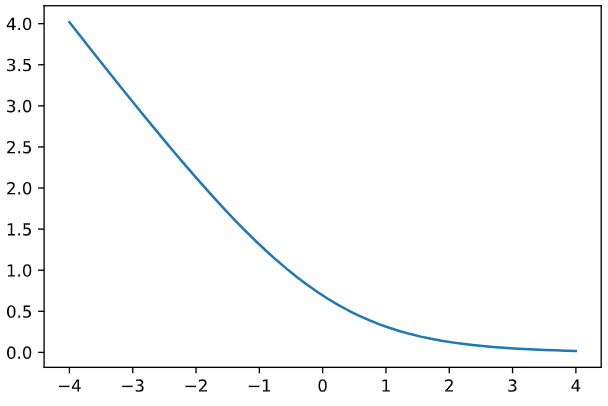
\includegraphics{plots/logistic_loss.png}}
      \tiny{\\Kolter \& Madry, 2019}
    \end{figure}
  \end{itemize}

\framebreak

  \begin{itemize}
    \item Maximizing such a monotonically decreasing function is equivalent to minimizing the argument.
    \lz
    \item Therefore
          \begin{align*}
            \max_{\deltab \in \Delta(\xv)} \Psi(y (\thetab^T(\xv + \deltab) + \theta_0)) &= \Psi(\min_{\deltab \in \Delta(\xv)}y (\thetab^T(\xv + \deltab) + \theta_0)) \\
                                                                                    &= \Psi (y (\thetab^T\xv + \theta_0) + \min_{\deltab \in \Delta(\xv)} y (\thetab^T \deltab))
          \end{align*}
    \lz
    \item We have to solve the problem
    $$ \min_{\deltab \in \Delta} y (\thetab^T \deltab) $$
  \end{itemize}

\framebreak

  \begin{itemize}
    \item To get a feel for the problem, let us consider the case where $y = +1$ and use $\Delta = \mathcal{B}^{\infty}_{\epsilon}$. The latter constrains each element of $\delta$ to lie between $-\epsilon$ and $+\epsilon$.
    \lz
    \item The quantity $y (\thetab^T \deltab)$ is then minimized when $\delta_j = - \epsilon$ for $\theta_{j} \geq 0$ and $\delta_j = \epsilon$ for $\theta_{j}<0$.
    \lz
    \item For $y = -1$, the signs would be flipped.
    \lz
    \item The optimal solution then, is
    $$\deltab^* = -y\epsilon \cdot \sign(\thetab) $$
    \item Note that the optimal solution does not explicitly depend on $\xv$. 

\framebreak

  \item The function value achieved by the solution is: 
  $$y \cdot \thetab^T \deltab^* = y \cdot \sum_j -y \epsilon \cdot \sign(\theta_j)\theta_j = - y^2 \epsilon \sum_j | \theta_j | = -\epsilon\|\thetab\|_{1} $$
  \item Therefore, we have analytically computed the solution to the inner maximization problem! The solution is:
  $$ \max_{\deltab \in \Delta(\xv)} \Psi(y (\thetab^T(\xv + \deltab) + \theta_0)) =  \Psi (y (\thetab^T(\xv + \deltab)) -\epsilon\|\thetab\|_{1}) $$
  \item As a result, the adversarial risk, which was a min-max problem, has now been converted to a pure minimization problem:
  $$\min_{\thetab, \theta_0} \frac{1}{N} \sum_{i = 1}^{N} \Psi \left(\yi \cdot\left(\thetab^{T} \xi +\theta_0\right)-\epsilon\|\thetab\|_{1}\right)$$
  \item This problem is convex in $\{\thetab, \theta_0\}$ and can be solved exactly. An iterative optimizer such as SGD will also approach the global minimum.
  \end{itemize}
  
\end{vbframe}

\begin{vbframe} {MNIST example}

  \begin{itemize}
    \item As an example, we look at the MNIST dataset, but this time we perform logistic regression and focus only on the classification of 0s vs.    1s.
    \lz
    \item The logistic regression classifier was trained for 10 epochs with SGD on the training set. 
    \lz
    \item This model obtained a low misclassification rate of 0.0004 on the test set.  
    \lz
    \item To generate adversarial examples, $\Delta$ is defined as $\mathcal{B}^{\infty}_{0.2}$.
    \lz
    \item As we saw earlier, the optimal perturbation $\deltab^*$ is $-y\epsilon \cdot \sign(\thetab)$.
  \framebreak
  \item As $\deltab^*$ does not directly depend on $\xv$, it is the "same" (ignoring the value of label $y$) across all examples. This is what it looks like:
    \begin{figure}
    \captionsetup{font=footnotesize,labelfont=footnotesize, labelfont = bf}
    \centering
      \scalebox{0.23}{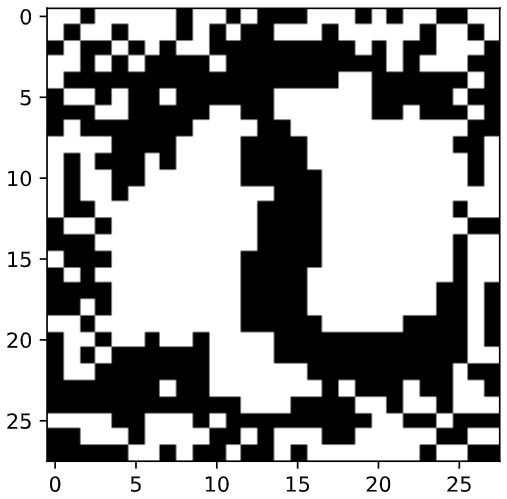
\includegraphics{plots/perturbation.png}}
      %\tiny{\\Credit: Kolter and Madry}
      \caption{The optimal perturbation for images that contain 0. For images that contain 1, the signs would be flipped (Kolter \& Madry, 2019). (The contrast between the black and white pixels is amplified for the sake of visualization.) }
    \end{figure}
    \item The perturbation (\textit{vaguely}) has a vertical line (like a 1) in black pixels, and a circle (like a 0) in white pixels. Intuition: When a given image is moved (translated) in the black direction, it is more likely to be classified as 1, whereas when moved in the white direction, it is more likely to be classified as 0.
 
    \framebreak
    
    \begin{figure}
    \centering
    \captionsetup{font=footnotesize,labelfont=footnotesize, labelfont = bf}
      \scalebox{0.6}{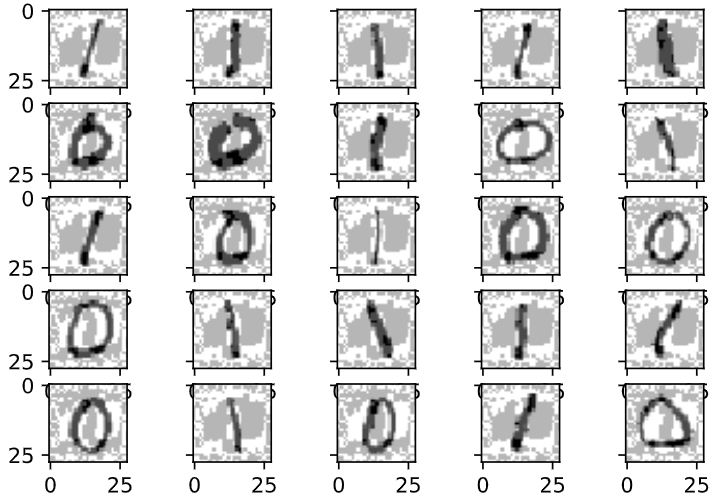
\includegraphics{plots/perturbed.png}}
      %\tiny{\\Credit: Kolter and Madry}
      \caption{Perturbed images from the test set (Kolter \& Madry, 2019).}
    \end{figure}
    
      \item \small{When all the images in test set are perturbed, the misclassification error of the model jumps from 0.0004 to 0.845!
      \item Interestingly, when the model is trained on similarly perturbed images from the training set (that is, the empirical adversarial risk is minimized), the misclassification error on the perturbed test set drops to 0.025.}
    \end{itemize}
    \framebreak
  
  % \begin{itemize}
  %   \item Robust training
  % \end{itemize}
  % 
  % \framebreak
  
    % \begin{figure}
    % \captionsetup{font=footnotesize,labelfont=footnotesize, labelfont = bf}
    % \centering
    %   \scalebox{0.8}{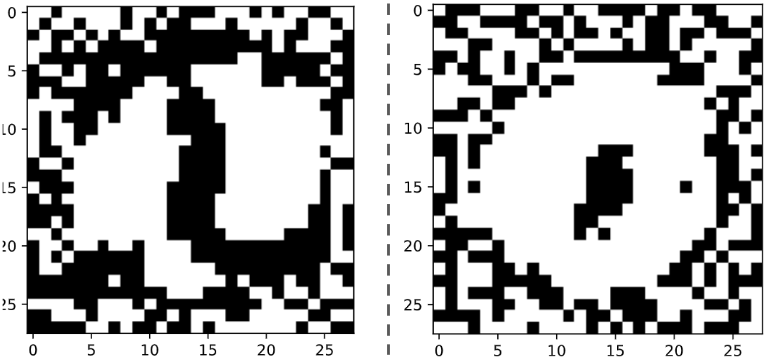
\includegraphics{plots/rob_perturbation.png}}
    %   \tiny{\\source: https://adversarial-ml-tutorial.org/}
    %   \caption{???}
    % \end{figure}
  
\end{vbframe}


%%%%%%%%%%%%%%%%%%%%%%%%%%%%%%%%%%%%%%%%%%%%%%%%%%%%%%%%%%%%%%%%%%

%%%%%%%%%%%%%%%%%%%%%%%%%%%%%%%%%%%%%%%%%%%%%%%%%%%%%%%%%%%%%%%%%%
%%%%%%%%%%%%%%%%%%          REFERENCES          %%%%%%%%%%%%%%%%%%
%%%%%%%%%%%%%%%%%%%%%%%%%%%%%%%%%%%%%%%%%%%%%%%%%%%%%%%%%%%%%%%%%%
%\section{References}
\begin{vbframe}
\frametitle{References}
\footnotesize{
\begin{thebibliography}{99}
%%%%%%%%%%%%%%%%%%%%%%%%%%%%%%%%%%
\bibitem[Kolter and Madry (2019)]{1} Zico Kolter and Aleksander Madry (2019)
\newblock Adversarial Robustness - Theory and Practice
\newblock \emph{\url{https://adversarial-ml-tutorial.org/}}
%%%%%%%%%%%%%%%%%%%%%%%%%%%%%%%%%%
\bibitem[Goodfellow et al., 2016]{1} Ian Goodfellow, Yoshua Bengio and Aaron Courville (2016)
\newblock Deep Learning
\newblock \emph{\url{http://www.deeplearningbook.org/}}
%%%%%%%%%%%%%%%%%%%%%%%%%%%%%%%%%%
\bibitem[Goodfellow, 2017]{1} Ian Goodfellow (2017)
\newblock Lecture 16 | Adversarial Examples and Adversarial Training
\newblock \emph{\url{https://www.youtube.com/watch?v=CIfsB_EYsVI}}
%%%%%%%%%%%%%%%%%%%%%%%%%%%%%%%%%%
\bibitem[Goodfellow et al., 2017]{1}  Ian GoodfellowNicolas PapernotSandy HuangRocky DuanPieter AbbeelJack Clark (2017)
\newblock Attacking Machine Learning with Adversarial Examples
\newblock \emph{\url{https://openai.com/blog/adversarial-example-research/}}
%%%%%%%%%%%%%%%%%%%%%%%%%%%%%%%%%%
% \bibitem[Hastie et al., 2009]{2} Trevoe Hastie, Robert Tibshirani and Jerome Friedman (2009)
% \newblock The Elements of Statistical Learning
% \newblock \emph{\url{https://statweb.stanford.edu/\%7Etibs/ElemStatLearn/}}
% %%%%%%%%%%%%%%%%%%%%%%%%%%%%%%%%%%
\bibitem[Nguyen et al., 2015]{1} Anh Nguyen, Jason Yosinski and Jeff Clune (2015)
\newblock Deep Neural Networks are Easily Fooled: High Confidence Predictions for Unrecognizable Images
\newblock \emph{\url{https://arxiv.org/abs/1412.1897}}
%%%%%%%%%%%%%%%%%%%%%%%%%%%%%%%%%%
\bibitem[Krizhevsky et al., 2012]{1} Alex Krizhevsky, Ilya Sutskever and Geoffrey E. Hinto (2012)
\newblock ImageNet Classification with Deep Convolutional Neural Networks. NIPS. 
\newblock \emph{\url{https://papers.nips.cc/paper/4824-imagenet-classification-with-deep-convolutional-neural-networks}}
%%%%%%%%%%%%%%%%%%%%%%%%%%%%%%%%%%
% \bibitem[Hinton et al., 2012]{3} Geoffrey E Hinton, Nitish Srivastava, Alex Krizhevsky Ilya Sutskever and Ruslan Salakhutdinov (2012)
% \newblock Improving neural networks by preventing co-adaptation of feature detectors
% \newblock \emph{\url{http://arxiv.org/abs/1207.0580}}
% %%%%%%%%%%%%%%%%%%%%%%%%%%%%%%%%%%
\bibitem[Maxence Prevost (2018)]{1} Maxence Prevost (2018)
\newblock Adversarial ResNet50 
\newblock \emph{\url{http://arxiv.org/abs/1207.0580}}
%%%%%%%%%%%%%%%%%%%%%%%%%%%%%%%%%%
\bibitem[Sharif et al. (2016)]{1} Mahmood Sharif, Sruti  Bhagavatula and Lujo Bauer (2016)
\newblock Accessorize to a Crime: Real and Stealthy Attacks onState-of-the-Art Face Recognition. Proceedings of the 2016 ACM SIGSAC Conference on Computer and Communications Security.
\newblock \emph{\url{https://dl.acm.org/doi/10.1145/2976749.2978392}}
%%%%%%%%%%%%%%%%%%%%%%%%%%%%%%%%%%
\bibitem[Goodfellow et al., 2014]{5} Goodfellow, Shlens (2014)
\newblock Explaining and Harnessing Adversarial Examples
\newblock \emph{\url{https://github.com/maxpv/maxpv.github.io/blob/master/notebooks/Adversarial_ResNet50.ipynb}}
%%%%%%%%%%%%%%%%%%%%%%%%%%%%%%%%%%
\bibitem[Papernot et al., 2016]{5} Papernot , McDaniel, Goodfellow, Jha, Celik, Swamy (2016)
\newblock Practical Black-Box Attacks against Machine Learning
\newblock \emph{\url{https://arxiv.org/abs/1602.02697}}
%%%%%%%%%%%%%%%%%%%%%%%%%%%%%%%%%%
\bibitem[Athalye et al., 2017]{5} Athalye , Engstrom, Ilyas, Kwok (2017)
\newblock Synthesizing Robust Adversarial Examples
\newblock \emph{\url{https://arxiv.org/abs/1707.07397}}
%%%%%%%%%%%%%%%%%%%%%%%%%%%%%%%%%%
\bibitem[Brown et al., 2018]{1} Tom B. Brown and Catherine Olsson, Research Engineers, Google Brain Team (2018)
\newblock 
Introducing the Unrestricted Adversarial Examples Challenge 
\newblock \emph{\url{https://ai.googleblog.com/2018/09/introducing-unrestricted-adversarial.html}}
%%%%%%%%%%%%%%%%%%%%%%%%%%%%%%%%%%
\end{thebibliography}
}
\end{vbframe}
%%%%%%%%%%%%%%%%%%%%%%%%%%%%%%%%%%%%%%%%%%%%%%%%%%%%%%%%%%%%%%%%%%
%%%%%%%%%%%%%%%%%%%%%%%%%%%%%%%%%%%%%%%%%%%%%%%%%%%%%%%%%%%%%%%%%%
\endlecture
\end{document}
